\documentclass{article}

\linespread{1.5}
\usepackage[utf8]{inputenc}
\usepackage[left=1.5in,right=1.5in,bottom=1in]{geometry}
\setlength\parindent{0pt}
\setlength{\parskip}{1em}
\setcounter{secnumdepth}{0}
\usepackage{outlines}
\usepackage{graphicx}
\graphicspath{ {imgs} }
\usepackage{hyperref}
\usepackage{color,soul}
\usepackage[normalem]{ulem}

\usepackage[
backend=biber,
style=apa,
citestyle=authoryear,
sorting=nyt,
]{biblatex}
\addbibresource{refs.bib}

\usepackage{comment}
\specialcomment{topicsen}{\begingroup\bfseries\scriptsize}{\endgroup}
%\excludecomment{topicsen}

\newcommand{\alignedmarginpar}[1]{%
        \marginpar{\raggedright\small #1}
    }

\title{Contemporary Challenges in Urban Development}
\author{Carla Hyenne}

\begin{document}

\maketitle

\tableofcontents

\pagebreak

\section{Introduction to Sustainable Urban Development}

\section{}

\subsection{Seestadt Aspern}

Notes from excursion:

\begin{outline}
	\1 Pillars: renewable energy, use of green space, inclusion;
	\1 Seestadt Aspern tries to tackles challenges that were present in Vienna. Aiming to provide affordable housing, approx. 60\% of people in Vienna live in social or some type of subsidised housing.

\end{outline}

Collective thoughts on the excursion:

\begin{outline}
	\1 Dystopian but nice: on the fringes of the development, the space feels dystopian and not inviting; but in the centre of the built area, it was lived in and people were out and using the spaces
	\1 Familiarity: feeling of having seen these spaces, because they look like any other modern developments
	\1 Public participation: a lot of involvement from residents, and a lot of input to be given since everything is being built from scratch
	\1 Ground floor usage: regulated ground space: many spaces for recreation, but still regulated; some spaces can be used as playgrounds, but not for football
	\1 Narratives: there are no/limited authentic places, with local (Viennese, Austrian) or foreign shops (Turkish)
	\1 Linkages: the blocks felt like they could exchanged with another, and therefor the plots don't seem to have relation or strong links with one another; how do you motivate people to interact and belong in this space?
	\1 What isn't there? No irregularity or surprises, nothing unexpected that happens - the narrative is narrow, which doesn't happen often in cities
\end{outline}

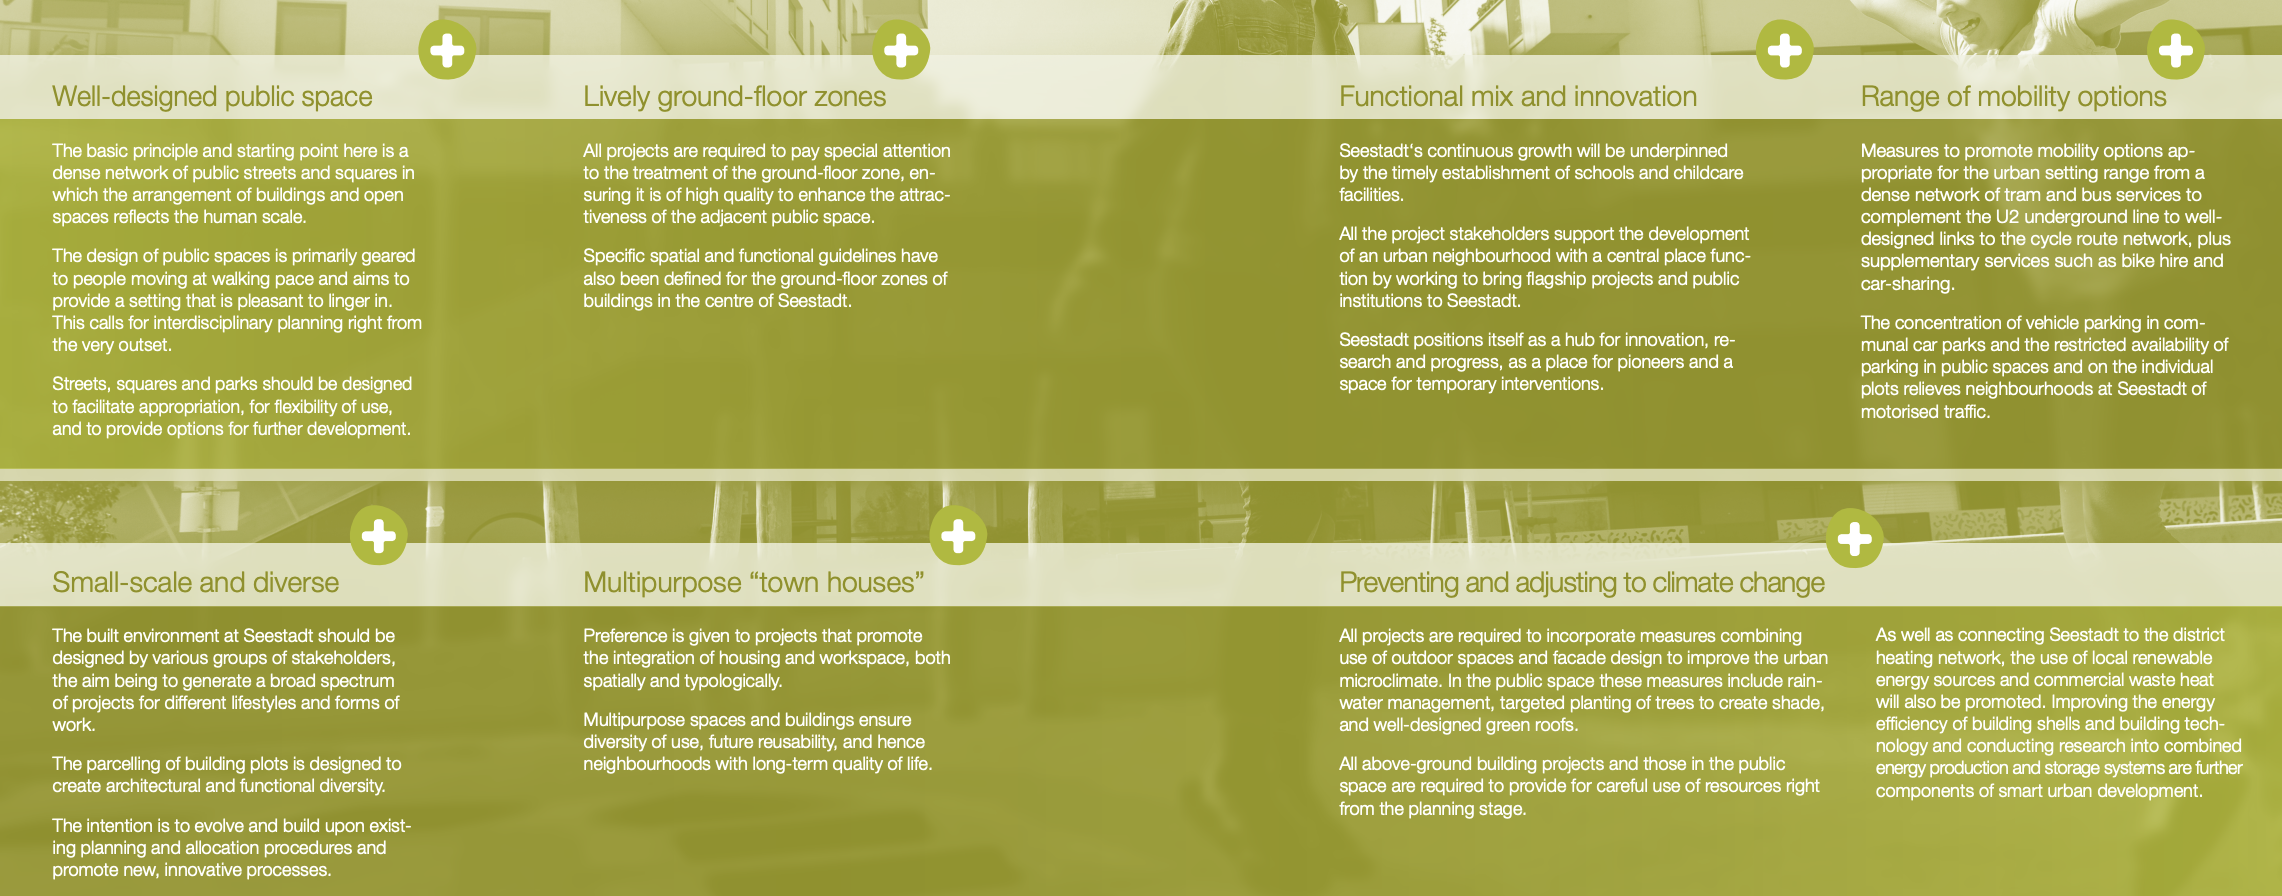
\includegraphics[width=\textwidth]{seestadt_quality_criteria}

\subsubsection{Urban Innovation Vienna}

\textit{Mag. Herbert Bartik}

Urban Innovation Vienna is a development agency working on Seestadt Aspern. They are building the frameworks and indicators for the development, and conduct an evaluation, but they are not making decisions as to what is built or the decisions made - more recommendations.

Seestadt development started in 2014, and is at half time (another 9 or so years until it is completed). Good time to evaluate past performance and future plans. What has been learnt, what goals should be integrated in to the future development, and what features have to be intensified to reach the goals?

\begin{outline}
	\1 Strategy pyramid:
		\2 Strategies of Seestadt: smart city strategy of Vienna, sustainability road map
		\2 Sectoral strategies
		\2 Thematic concepts (mobility)
\end{outline}

Other case studies: Paris, London, Berlin, Hamburg. In the UK, cities are required by federal law to provide the KPIs.\alignedmarginpar{Kings X Central}

Affordability is built in to the plan, but not an excuse for developing on the goals. This aspect of affordability is particular to the city of Vienna, which is known for its affordable housing, in comparison to other big cities who have comparable urban development sites - they all have goals of affordability, but not on the same level or focus (is Kings X Central affordable??). The point in looking at other projects in other cities, is not to compare but to be inspired by. 

To what extent are the Seestadt quality criteria of the master plan considered in the framework?

What about evaluation frameworks outside of planning?

\subsection{Why Indicators?}

Indicators are used to evaluate how sustainable a development, like Seestadt Aspern, is.

Indicators break down space into measurable units, into something quantifiable, reducing the complexity into metrics. Used to contextualise goals, for the assessment/evaluation/monitoring, to set targets and measure progress, to compare, as communication tools and evidence for decision-making. The goals of indicators are to be Specific, Measurable, Attainable, Relevant, Timely.

Indicators can be bundled into composite indicators. An index (indices) are an aggregation of multiple indicators, along with normalisation, weighting, aggregation and sensitivity analysis.

\subsubsection{Measuring sustainability}

Frameworks: SDG Interaction trade-offs and co-benefits

How to measure sustainability, and transformations? New tools required other than purely data-driven indicators, avoid ``greening'' by numbers (eg. measuring environmental parameters with smart technologies), focus on numbers hides effects (eg. increase in green spaces can lead to inclusion), ``living'' indicators (eg. impacts on social movements). $\rightarrow$ ref. \parencite{kaika2017don}

\subsubsection{CITYKeys}

Five dimensions: People, Planet, Prosperity ,Governance, Propagation. What are the `smart city' aspects of each dimension?

From 43 sets of indicators, then added 25 indicators, and out of the 99 project indicators, only 20 can be quantitatively used on the city level. 

\section{Coursework}

$\rightarrow$ developing indicators for the criteria selected


\end{document}
